%!TEX program = xelatex
\documentclass[12pt]{ctexart}
\usepackage{geometry}
\usepackage{enumitem}
\usepackage{tikz}
\usepackage{amsmath}
\usepackage{float}

\usepackage{fancyhdr}
 
\pagestyle{fancy}
\fancyhf{} % 清除所有页眉和页脚的默认设置
\renewcommand{\headrulewidth}{0pt} % 如果不需要页眉横线,可以设置为0pt
\renewcommand{\footrulewidth}{0pt} % 如果不需要页脚横线,可以设置为0pt
\fancyfoot[C]{\thepage} % 将页码放置在页脚中央

\geometry{a4paper, margin=2cm}


\begin{document}

\section*{小学五年级奥林匹克数学竞赛试卷}

\subsection*{第一部分:选择题}
\begin{enumerate}[label=\arabic*., left=0pt]
\item 小明买书,如果按原价的80\%支付,节省了12元。书的原价是多少元?
\newline
\hspace*{0.5cm} A. 60元 \hfill B. 75元 \hfill C. 80元 \hfill D. 90元

\item 观察数列:2, 5, 10, 17, 26, … 下一个数是多少?
\newline
\hspace*{0.5cm} A. 33 \hfill B. 35 \hfill C. 37 \hfill D. 39

\item 如图,两个正方形组成一个组合图形,边长分别为4厘米和3厘米,这个组合图形的周长是多少?
\begin{figure}[H]
\flushright
\begin{tikzpicture}[scale=0.5]
\draw (0,0) -- (4,0) -- (4,4) -- (0,4) -- cycle;
\draw (4,1) -- (7,1) -- (7,4) -- (4,4) -- cycle;
\node at (2,0) [below] {4厘米};
\node at (5.5,1) [below] {3厘米};
\end{tikzpicture}
\end{figure}
\vspace{2cm}
\hspace*{0.5cm} A. 22厘米 \hfill B. 24厘米 \hfill C. 26厘米 \hfill D. 28厘米

\item 下列几何体中,哪一个与其他三个不同类?
\newline
\hspace*{0.5cm} A. 正方体 \hfill B. 长方体 \hfill C. 棱锥 \hfill D. 圆柱

\item 甲乙两人从相距50公里的两地相向而行,甲的速度是6公里/小时,乙的速度是4公里/小时。甲带了一条狗,狗以10公里/小时的速度在两人之间往返奔跑。当甲乙相遇时,狗一共跑了多少公里?
\newline
\hspace*{0.5cm} A. 40公里 \hfill B. 50公里 \hfill C. 60公里 \hfill D. 70公里
\end{enumerate}

\subsection*{第二部分:解答题}
\begin{enumerate}[label=\arabic*., left=0pt]
\item 鸡兔同笼,共有头20个,脚56只。问鸡和兔各有多少只?
\begin{figure}[H]
\flushright
\begin{tikzpicture}[scale=0.4]
\draw (0,0) circle (1cm);
\draw (3,0) circle (1cm);
\draw (-2, -2) rectangle (5, 2);
\node at (0,0) {鸡};
\node at (3,0) {兔};
\end{tikzpicture}
\end{figure}
\vspace{4cm}

\item 将一个边长为5厘米的正方形分成四个相同的小长方形,每个小长方形的周长都是15厘米。求每个小长方形的长和宽。
\begin{figure}[H]
\flushright
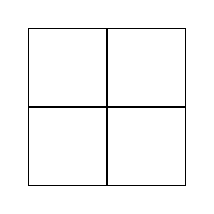
\begin{tikzpicture}[scale=0.4]
\draw (0,0) -- (5,0) -- (5,5) -- (0,5) -- cycle;
\foreach \x in {2.5} {
    \draw (\x,0) -- (\x,5);
    \draw (0,\x) -- (5,\x);
}
\end{tikzpicture}
\end{figure}
\vspace{4cm}

\item 如图,等腰直角三角形ABC的腰长为6厘米,以斜边为直径作半圆。求阴影部分的面积(取π=3.14)。
\begin{figure}[H]
\flushright
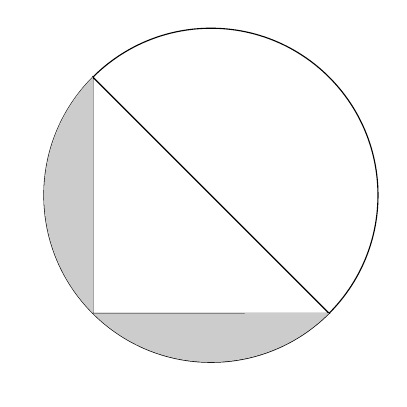
\begin{tikzpicture}[scale=0.5]
\draw (0,0) -- (6,0) -- (0,6) -- cycle;
\draw (3,3) circle (3*1.414);
\fill[gray!40] (0,6) arc (135:315:4.24) -- (0,0) -- cycle;
\end{tikzpicture}
\end{figure}
\vspace{4cm}
\end{enumerate}

\newpage
\section*{参考答案}

\subsection*{选择题}
\begin{enumerate}[label=\arabic*., left=0pt]
\item A
\item C
\item C
\item D
\item B
\end{enumerate}

\subsection*{解答题}
\begin{enumerate}[label=\arabic*., left=0pt]
\item 鸡有12只,兔有8只。
  
  设鸡有$x$只,兔有$y$只:
  \[
  \begin{cases}
  x + y = 20 \\
  2x + 4y = 56
  \end{cases}
  \]
  解得:$y=8$, $x=12$

\item 每个小长方形的长为5厘米,宽为2.5厘米。
  
  设长方形长为$a$,宽为$b$,由周长公式:
  \[
  2(a + b) = 15 \Rightarrow a + b = 7.5
  \]
  根据正方形分割方式可得:$a=5$厘米,$b=2.5$厘米

\item 阴影部分面积为 $10.26$ 平方厘米。
  
  斜边长:$\sqrt{6^2+6^2}=6\sqrt{2}$ 厘米 \\
  半圆面积:$\frac{1}{2} \pi (3\sqrt{2})^2 = 28.26$ 平方厘米 \\
  三角形面积:$\frac{1}{2} \times 6 \times 6 = 18$ 平方厘米 \\
  阴影面积:$28.26 - 18 = 10.26$ 平方厘米
\end{enumerate}

\end{document}